\documentclass{article}
\usepackage{fontspec}
\usepackage{polyglossia}
\usepackage{pgfplots}
\usepackage{tikz}
\usepackage{unicode-math}
\usepackage{amsmath}
\usepackage{listings}
\usepackage{algorithm}
\usepackage{algpseudocode}
\usepackage{subfig}

\usetikzlibrary{patterns}

\setmainlanguage{french}

\newcommand{\R}{\mathbb{R}}

\DeclareMathOperator{\card}{card}
\DeclareMathOperator{\argmax}{argmax}
\DeclareMathOperator{\uniform}{Uniform}

\title{Ocaml---IA\\Tetris par Qlearning}
\author{C.~Cousin, G.~Hondet, L.~Pineau, B.~Viry}
\date{\today}


\begin{document}
\maketitle
\tableofcontents

\section*{Introduction}

\section*{Notations}
Seront not\'es dans tout l'ouvrage:
\begin{itemize}
  \item \(n_t\) le nombre de tetrominos par jeu,
  \item \(\mathcal{S}\) l'ensemble des \'etats,
  \item \(b_w, b_h\) la largeur et la hauteur totale du plateau.
\end{itemize}
Sauf mention explicite, les applications utiliseront les valeurs \(n_t=10,000,
b_w = 6\). Seront distingu\'ees la hauteur totale \(b_h\) et la hauteur relative
à un instant de jeu \(h\) du plateau, la première correspond à la hauteur
théorique maximale atteignable quand la deuxieme concerne la hauteur
effectivement atteinte à un instant de jeu, i.e.\ le nombre de lignes non vides
sur le plateau.

\section{Tetris}

\subsection{Le jeu et sa simplification}
Tetris met le joueur au défi de réaliser des lignes complètes en déplaçant des
pièces de formes différentes, les tétrominos, qui défilent depuis le haut
jusqu'au bas de l'écran. Les lignes complétées disparaissent tout en rapportant
des points et le joueur peut de nouveau remplir les cases libérées. Le jeu
n'a pas de fin: le joueur perd la partie lorsqu'un tétrimino reste bloqué en
haut.

Dans notre version simplifiée, il n'y a pas de limite de hauteur, le jeu se
termine apres avoir fourni 10,000 tetrominos à placer. De plus notre
tetris diffère par une grille plus étroite (6 colonnes disponibles), moins de
tetrominos différents (seulement 5) et des tetrominos plus petits (taille
inférieure à 2).

Un tetromino est plac\'e par le choix d'une colonne et d'une orientation.

\subsection{L'impl\'ementation}

\subsubsection{Représentation}

\paragraph{Tetrominos}
Les tetrominos sont tableaux de longueur 4. L'unidimensionnalit\'e permet
d'impl\'ementer les rotations comme des transformations d'indices, \'evitant la
cr\'eation ou la modification de structures.

IMAGE NED EED\\
Les tetrominos sont tous de même dimension par souci d'homogénéite.

\paragraph{Plateau \texttt{Board}}
Le plateau est repr\'esent\'e par une matrice de dimension
\(2\cdot n_t\cdot 6\) d'entiers dans laquelle on inscrit les tetrominos. Les
manipulations du plateau se font en place.


\paragraph{Actions}
Composées d'une rotation et d'une translation. Elles permettent d'agir sur les
tetrominos. Les rotations sont representées par les points cardinaux
(North, South, East, West) et les translations par un entier compris entre 0 et
4 correspondant à l'indice du coin supérieur gauche du tetromino.
\begin{figure}
  \centering
  \subfloat[Diagonale] {%
    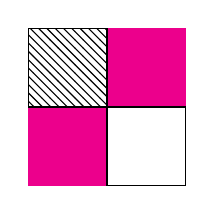
\begin{tikzpicture}
      \fill[color=magenta] (0,0) rectangle (1,1);
      \fill[color=magenta] (0,0) rectangle (-1,-1);
      \draw[pattern = north west lines] (0,0) rectangle (-1,1);
      \draw (0,0) rectangle (1,-1);
    \end{tikzpicture}
  }\qquad
  \subfloat[L] {%
    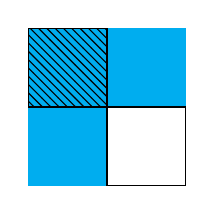
\begin{tikzpicture}
      \fill[color=cyan] (0,0) rectangle (1,1);
      \fill[color=cyan] (0,0) rectangle (-1,-1);
      \fill[color=cyan] (0,0) rectangle (-1,1);
      \draw[pattern = north west lines] (0,0) rectangle (-1,1);
      \draw (0,0) rectangle (1,-1);
    \end{tikzpicture}
  }
  \caption{Point de reference de tetromini, ici hachure}\label{fig:tetref}
\end{figure}

La geometrie de certains tetromini rend certaines orientations redondantes. Par
exemple le carre est invariant par rotation, et utiliser les quatre rotations
ne fait qu'augmenter inutilement le nombre d'actions possibles, et augmente par
consequent la quantite d'information que l'agent doit apprendre. Pour pallier
cette redondance, chaque tetromino dispose de son propre ensemble de rotations
applicables.

\subsection{D\'eroulement d'une partie}
Lors d'une partie le joueur doit poser les pièces qui lui sont proposées sur
le plateau de jeu. Il est donc nécessaire d'utiliser une fonction \texttt{play}
qui permet de placer une pièce sur le plateau. La pièce ``tombe'' donc dans la
colonne sélectionnée tant qu'elle ne rencontre pas d'obstacle (fond du plateau
ou un autre tétromino). Pour cela, il y a besoin d'une fonction de test de
collision, qui renvoie si l'emplacement testé peut accueillir le tetromino.
S'il y a collision, on sélectionne le dernier emplacement libre et on place la
pièce.

Lorsqu'une ligne est entièrement remplie, elle est supprimée du tableau, mais
la taille totale du plateau reste la même.

\subsection{Drawbacks}
\subsubsection{Fonction collide}
L'implémentation actuelle oblige l'accessibilit\'e de la position finale depuis
le haut du plateau car la pi\`ece ne peut pas \^etre gliss\'ee au dernier moment
sous une autre.
\subsubsection{Tetromino}
Les tetrominos sont tous de même dimension par souci d'homogénéite et cela
peut entrainer un probleme de ``tetromino flottant''. Ce problème est traité par
un choix d'action spécifique à chaque pièce (cf partie x).
\section{Q learning}

\subsection{Représentation des états}
\subsubsection{Composition}
Intuitivement, un état correspond à la pièce donnée à jouer et la disposition
des pièces sur le plateau. En notant \(n_t\) le nombre de tetrominos et \(w\) la
largeur du plateau, on obtient \(5 \cdot 2^{wn_t}\) états possibles.

Pour réduire le nombre d'états, on ne considère que les deux plus hautes lignes
contenant au moins un tetromino. On obtient \(5\cdot 2^{w+1}\) états possibles,
soit \(20,480\) pour une largeur de 6.

\subsubsection{Codage}
Comme chaque état correspond \textit{in fine} à une ligne de la matrice, il est
nécessaire d'avoir une bijection entre l'ensemble des états et les entiers. La
bijection genère deux représentations entières, une pour les deux lignes de
l'état et l'autre pour la pièce et les combine en un état entier final,
\[
  \texttt{get\_state}\colon [0,4]\times [0, 2^{12} - 1] \to [0, 5\cdot 2^{12}].
\]


\subsection{Algorithmes}

L'algorithme~\ref{alg:action} concerne la maniere dont l'agent choisit les
actions parmi l'ensemble des actions possibles \(\mathcal{A}\), etant donne un
etat \(s\). Le parametre \(\epsilon\) definit la frequence de choix aleatoire.
\begin{algorithm}
  \caption{Choix de l'action}\label{alg:action}
  \begin{algorithmic}
    [1]
    \Procedure{ChooseAction}{$Q$, $s$, $\mathcal{A}$}
    \State{} tirage \(\gets \uniform([0, 1])\)
    \If{tirage \(> \epsilon\)}
    \Return{\(\argmax_{a\in\mathcal{A}} Q(s, a)\)}\Comment{Choix de l'action
    maximisant l'esperance de recompense}
    \Else{}
    \Return{\(\uniform(\mathcal{A})\)}\Comment{Choix aleatoire}
    \EndIf{}
    \EndProcedure{}
  \end{algorithmic}
\end{algorithm}


L'algorithme~\ref{alg:qlearning} definit la maniere dont l'agent se met a jour
afin de maximiser l'esperance de gain. Est notee \(\gamma\) la vision de
l'agent correspondant a l'importance que l'agent attribue aux recompenses
futures par rapport a la recompense immediate. Un \(\gamma\) de zero cree un
agent myope ne choisissant son action que par rapport a la recompense immediate
tandis qu'un \(\gamma\) tendant vers un associe autant d'importance aux
recompenses des coups suivants qu'a la recompense immediate.
\begin{algorithm}
  \caption{Algorithme de \textit{Q-learning}}\label{alg:qlearning}
  \begin{algorithmic}
    [1]
    \Procedure{Update}{$Q$, $\epsilon$, $\gamma$, $\alpha$}
    \Repeat{}
    \State{} initialisation de \(s\)
    \Repeat{}
    \State{} \(a \gets\) ChooseAction$(Q, s, \mathcal{A}, \epsilon)$
    \State{} jouer \(a\), observer \(r\) et le nouvel \'etat \(s'\),
    \State{} \(Q(s, a) \gets Q(s, a) + \alpha\left[ r + \gamma \max_{a'}
      Q(s', a') - Q(s, a)\right]\)
    \Until{$s$ est terminal}
    \Until{entrainement fini}
    \EndProcedure{}
  \end{algorithmic}
\end{algorithm}

\subsubsection{Param\`etres}
L'apprentissage est paramétré par les trois variables,
\begin{itemize}
  \item \(\alpha \in [0, 1]\) le taux d'apprentissage,
  \item \(\epsilon \in [0, 1]\) la fréquence de coups aléatoires effectués,
  \item \(\gamma \in [0, 1]\) la vision de l'agent.
\end{itemize}
Pour assurer la convergence de la matrice vers la matrice optimale,
le taux d'apprentissage doit évoluer au cours des entrainements.
D'après~\cite{watkins92}, la suite \( (\alpha_k)_k \) doit vérifier
\( \sum_{k=0}^\infty \alpha_k = \infty \) et \(
\sum_{k=0}^\infty \alpha_k^2 \in \R \). La suite choisie est donc, pour tout
\( k \in \mathbb{N} \) et avec \( C \in \R \)
\[
  \alpha_k = \frac{1}{1 + Ck}.
\]
Le taux d'apprentissage reste manipulable via le paramètre \( C \).


Le paramètre \(\epsilon\) pourra \'egalement varier au cours des jeux effectués.
En effet, intuitivement, un \(\epsilon\) grand permet une exploration rapide de
l'ensemble des états possibles mais devient nuisible lorsque la matrice est bien
entrainée.

\paragraph{Valeurs}
\begin{figure}
  \centering
  \begin{tikzpicture}
    \begin{axis}[only marks, mark size = 0.1,
        legend entries={0.80,0.84,0.88,0.92,0.96,1.00}
      ]
      \foreach \i in {0,1,...,5}{%
        \addplot+ table [x expr = {log2(\lineno)}, y index = \i] {data/gamma.dat};
      }
    \end{axis}
  \end{tikzpicture}
  \caption{Influence du parametre \(\gamma\)}
\end{figure}


\section{Difficultés rencontrées}

\subsection{Le fl\'eau de la mutabilit\'e}
L'usage du \texttt{Array.blit} s'est revélé plus delicat que prévu. En
considerant que la ligne \(l\) doit etre supprimée et en notant \(h\) la hauteur
actuelle du plateau, le principe est de copier la section de tableau incluant
les lignes \(l+1\) jusqu'à \(h+1\) une ligne en dessous, i.e.\ translater le
bloc d'une ligne vers le bas.

Cette démarche engendre des comportements anormaux car la ligne \(h+1\) n'est
pas copiée sur la ligne \(h\), elles partagent la même adresse mémoire. Ainsi,
il etait observé quelques coups après un blit un dédoublement de carrés de
tetrominos, faisant augmenter la hauteur.

Pour pallier ce problème de partage d'adresse mémoire, la ligne \(h\) est
recréée à chaque blit.

\subsection{Le hollandais volant}
La fonction collide permet de tester la collision du tetromino avec les autres
pièces et le fond du plateau. Lors de l'éxécution de la fonction \texttt{play}
on testait donc toutes les positions possibles pour déposer les pièces de
dimension 2 \(\times \) 2 sur le fond du plateau s'il n'y avait pas eu de
collision. Malheureusement, certaines pièces comme le point ou la ligne
pouvaient avoir une ``ligne vide'' en bas sous certaines rotations. Pour
résoudre ce problème qui est devenu évident après la résolution du problème de
\texttt{Array.blit}, nous avons décidé de restreindre les états possibles dans
la Q-matrice. En effet lors de l'initialisation de la Q-matrice, tous les états
accessibles sont mis à 0 (flottant) et tous les états non utilisés sont
initialisés à \(-\infty \). Ainsi, pour le point, on ne gardera que les
rotations \textt{South} et \textt{West}.

\section{R\'esultats du projet}

\section*{Conclusion}

\appendix
\section{Deep Q learning}

Pour s'affranchir de la limite de memoire due au nombre d'etats possibles, la
matrice est remplacee par une fonction lineaire, avec \(n \in \mathbb{N}, V
\colon \R^n \to \R\). En notant \(w = (w_0\, w_1\, \dots\, w_n)^\top\) les poids
de \(V\) et \(x = (x_1\, \dots\, x_n)\), \(V\) s'exprime
\[
  V \colon x \mapsto w_0 + \sum_{i=1}^n w_i x_i.
\]

La fonction \(V\) sera appliquee aux caracteristiques du plateau de jeu
(\textit{features} en anglais). Elles seront obtenues par le biais d'une
fonction \(\phi\colon \mathcal{S} \to \R^n\). Les caracteristiques utilisees
sont decrites dans~\cite{boumaza13}.
\begin{algorithm}
  \caption{Algorithme d'apprentissage d'une fonction lineaire}\label{alg:linfct}
  \begin{algorithmic}
    [1]
    \Procedure{Update}{$V$, $\epsilon$, $\gamma$, $\eta$, $\eta$}
    \Repeat{}
    \State{} initialisation de \(s\)
    \Repeat{}
    \For{1 to $B$}
    \State{} \(a \gets \mathup{ChooseAction}(V, s, \mathcal{A}, \epsilon)\)
    \State{} joue \(a\), observer \(r\) et le nouvel \'etat \(s'\)
    \State{} ajouter a la memoire \( \left(\phi(s), a, r, \phi(s')\right) \)
    \EndFor{}
    \State{} Chosir aleatoirement \(B\) quadruplets depuis la memoire
    \State{} \(y_t \gets r_t + \gamma V\left(\phi(s_t')\right)\)
    \State{} \(\delta_t \gets y_t - V \left(\phi(s_t)\right)\)
    \State{} \(\mathcal{L} \gets \frac{1}{2B}\sum_{k=1}^B \delta_t^2\)
    \State{} \(w \gets w - \eta \nabla_w \mathcal{L}\)
    \Until{$s$ est terminal}
    \Until{Entrainement fini}
    \EndProcedure{}
  \end{algorithmic}
\end{algorithm}

\begin{thebibliography}{9}
    \bibitem{watkins92}
    Christopher~J.C.H.~Watkins, Peter~Dayan,
    \textit{Q-Learning, Machine Learning}
    1992.
    \bibitem{deepmind}
    Voloddymyr~Mnih, Koray Kavukcuoghlu, David Silver, Alex Graves, Ioannis
    Antonoglou, Daan Wierstra, Martin Riedmiller,
    \textit{Playing Atari with Deep Reinforcement Learning}
    \bibitem{boumaza13}
    Amine Boumaza,
    \textit{How to design good Tetris players}
    2013.
\end{thebibliography}

\end{document}
